\begin{figure}

\centering

\begin{tikzpicture}

% Axes
\draw [->, thick] ( -1, 0 ) -- ++( 9, 0 );
\draw [->, thick] ( 0, -1 ) -- ++( 0, 7 );

% Regimes
\draw ( 0, 2 ) -- ++( 2, -2 );
\draw ( 1, 1 ) -- ++( 6, 0 );
\draw [dashed] ( 1, 1 ) -- ++( 4, 4 );
\draw ( 1, 1 ) -- ++( 6, 2 );
\draw ( 0, 2 ) -- ++( 6, 2 );

% Labels
\node at ( 0.5, 0.5 ) {I};
\node at ( 4.5, 0.5 ) {II};
\node at ( 4.5, 1.5 ) {III};
\node at ( 3.5, 2.5 ) {IV};
\node at ( 1.5, 3.5 ) {V};

\foreach \x in { 0, ..., 5 }
  \node at ( \x + 1, 0 ) [below] {\(10^\x\)};
\foreach \y in { 0, ..., 4 }
  \node at ( 0, \y + 1 ) [left] {\(10^\y\)};

\node at ( 3.5, -0.75 ) [below] {\(\dfrac{ L }{ \delta_f }\)};
\node at ( -0.75, 3.5 ) [left] {\(\dfrac{ u' }{ S_L }\)};

\node at ( 7, 1 ) [right] {\(S_L = u'\)};
\node at ( 7, 3 ) [right] {\(Ka = 1\)};
\node at ( 6, 4 ) [right] {\(Ka = 100\)};
\node at ( 5, 5 ) [above] {\(Da = 1\)};

\end{tikzpicture}

\caption[Borghi diagram]{The figure shows the Borghi diagram marking the various regimes of premixed turbulent combustion---I. laminar flames, II. wrinkled flamelets, III. corrugated flamelets, IV. thin flame zones, and V. broken reaction zones---separated by contours of Karlovitz number.}

\label{fig:borghiDiagram}

\end{figure}

